\begin{frame}{Schranken aus dem $B$-Zerfall}
\framesubtitle{Real- und Imaginärteil variabel}
	\begin{figure}
		\centering
		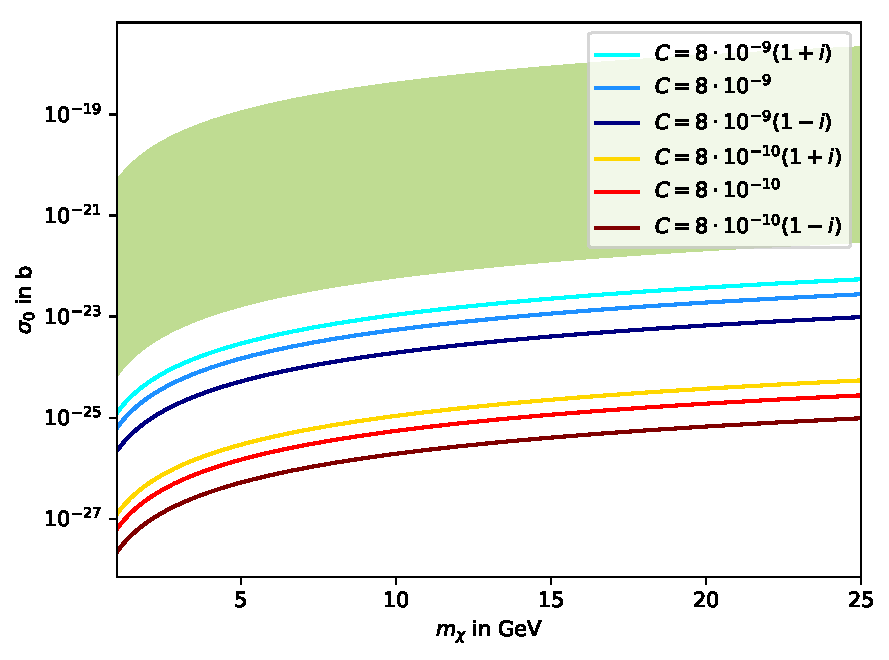
\includegraphics[width=.8\textwidth]{Bilder/Allgemein11.pdf}
		\caption{$q_l=q_\chi=1$}
	\end{figure}
\end{frame}
\begin{frame}[noframenumbering]{Schranken aus dem $B$-Zerfall}
\framesubtitle{Real- und Imaginärteil variabel}
	\begin{figure}
		\centering
		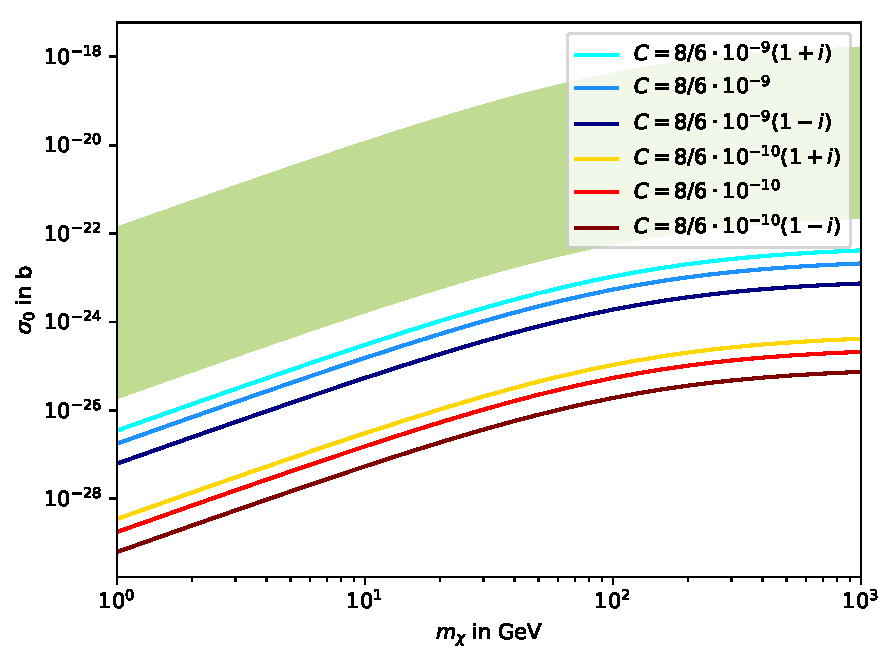
\includegraphics[width=.8\textwidth]{Bilder/Allgemein116.pdf}
		\caption{$q_l=1,q_\chi=\sfrac{1}{6}$}
	\end{figure}
\end{frame}


\begin{frame}{Schranken aus dem $B$-Zerfall}
\framesubtitle{Fester Realteil, variabler Imaginärteil}
	\begin{figure}
		\centering
		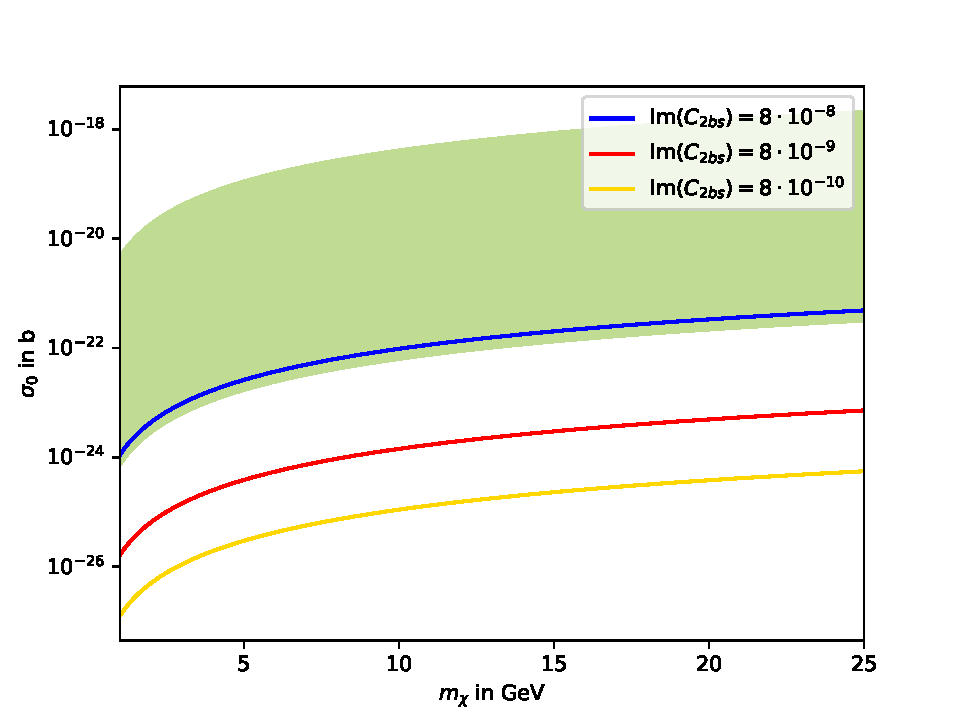
\includegraphics[width=.8\textwidth]{Bilder/Im11.pdf}
		\caption{$q_l=q_\chi=1$}
	\end{figure}
\end{frame}
\begin{frame}[noframenumbering]{Schranken aus dem $B$-Zerfall}
\framesubtitle{Fester Realteil, variabler Imaginärteil}
	\begin{figure}
		\centering
		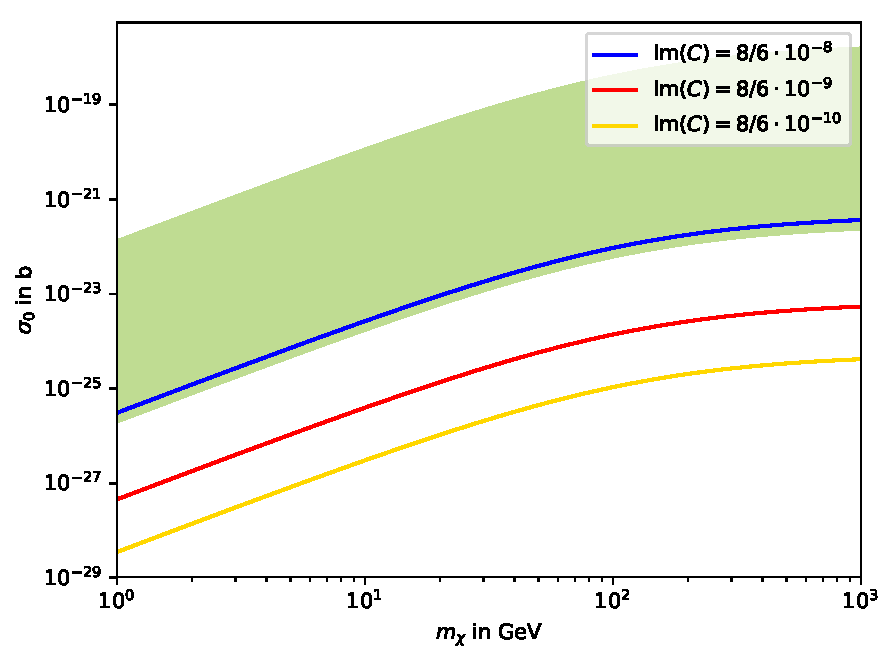
\includegraphics[width=.8\textwidth]{Bilder/Im116.pdf}
		\caption{$q_l=1,q_\chi=\sfrac{1}{6}$}
	\end{figure}
\end{frame}


\begin{frame}{Schranken aus der Relic Density}
\begin{figure}
	\centering
	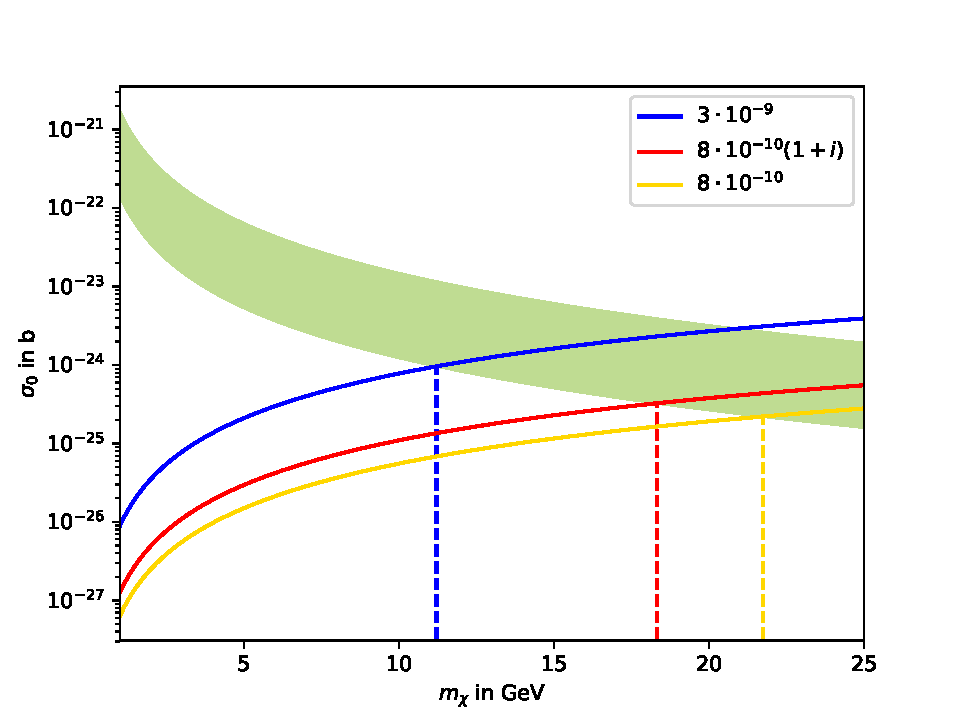
\includegraphics[width=.8\textwidth]{Bilder/Relic11.pdf}
	\caption{$q_l=q_\chi=1$}
\end{figure}
\end{frame}
\begin{frame}[noframenumbering]{Schranken aus der Relic Density}
\begin{figure}
\centering
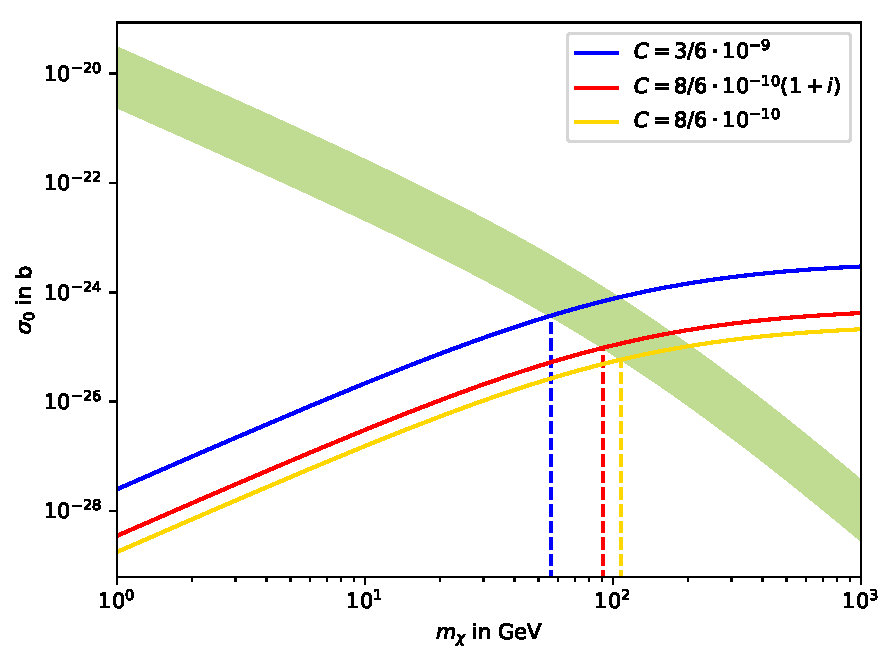
\includegraphics[width=.8\textwidth]{Bilder/Relic116.pdf}
\caption{$q_l=1,q_\chi=\sfrac{1}{6}$}
\end{figure}
\end{frame}